\section{Terrain Generation} \label{sec:system_architecture_terrain_generation}
The terrain was designed to randomly generate so that the player can have a new, unique map every time they play.
The second important part of the design was making sure that the player could edit the terrain in any way they wanted.
As described in \autoref{sec:theory_theory_marching_cubes} the marching cubes algorithm was chosen as the base of the terrain generation process.
This section will describe how we used this algorithm to generate the terrain and allow the player to edit it.

The algorithm consists of the following steps:
\begin{itemize}
    \item Define the scalar filed function.
    \item Divide the world into chunks.
    \item Generate the mesh.
\end{itemize}

Each of these steps will be described in detail in this section.

\subsection{Scalar Field} \label{subsec:scalar_field}
The first step in the terrain generation is to generate a scalar field which is a function that takes a point in 3D space and returns a value.
What is important is that this function always returns the same value for the same point.
Another important property is that the function should return close values for close points.
Our function returns values for points which have integer coordinates.

Having these properties in mind we decided to use the Perlin noise function.
Perlin noise first introduced by Ken Perlin in 1983 \cite{Perlin-Noise} is often used in computer graphics and in particular in procedural terrain generation.
It is a pseudo-random function that returns values for any point in 3D space.
\todo{Should we explain how the Perlin noise function works?}
However unlike some random functions it returns similar values for similar points.
This makes it ideal for this game.

The Perlin noise function is used to generate a value for each point in the scalar field.
This value is then modified based on 5 parameters: octaves, initial frequency, frequency multiplier, initial amplitude and amplitude multiplier.
These parameters are generate based on the seed of the world from 5 different sets of options which gives the game 5 terrains.
However we need more than just the value for each point and a normal vector.
Each point is also assigned a type based on the position that is later used to determine the type of the block which in turn determines its color.
\subsection{Chunks}
As mentioned before one of the most important thinks for the terrain was a way to edit it.
Editing the whole terrain at once would be very slow and not very efficient.
Thus the terrain is split into chunks - cubes with side length 16.
Each chunk is a separate object and can be edited independently.
This solution is much more efficient but is also causes some problems.

One problem is that the terrain is not continuous.
Every time we edit a chunk we need to make sure that the edges of the chunk are the same as the edges of the neighboring chunks.
This is done by making sure that when a function that updates one chunk is called it is also called with the exact same parameters for other affected chunks.
Without this the terrain would have holes in it between chunks which is shown in a screenshot from an early version of the game in \autoref{fig:gaps_between_chunks}.

Another problem is that the algorithm we used for generating the terrain, described in \autoref*{subsec:marching_cubes}, calculates normal vectors based on the values of the scalar field around the point at which the normal is calculated.
This means that that the normal vectors at the edges of the chunks have to be calculated differently.
This is a common problem with the algorithm and it is visualized in \autoref*{fig:problem_with_normals_at_chunk_edge}.
The most common solution and the one we used is extending the scalar field by one layer of points around the chunk.
This means that the chunk contains the information about the scalar field outside of the chunk itself.
That way the normal vectors can be calculated the same way for all points in the chunk.

\begin{figure}[H]
    \centering
    \begin{minipage}{0.45\textwidth}
        \centering
        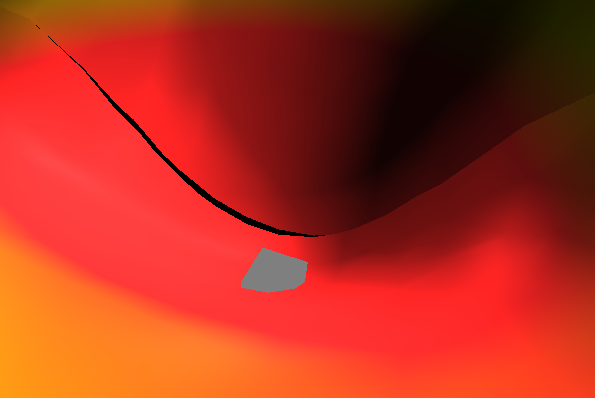
\includegraphics[width=0.8\textwidth]{chapters/system_architecture/sections/terrain_generation/resources/chunk_edges_gaps.png}
        \caption{Gaps between chunks.}
        \label{fig:gaps_between_chunks}
    \end{minipage}\hfill
    \begin{minipage}{0.45\textwidth}
        \centering
        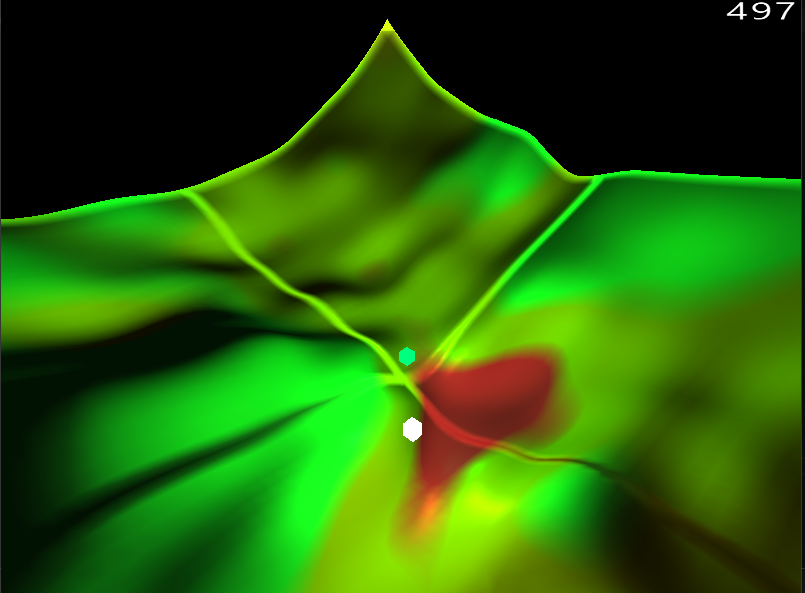
\includegraphics[width=0.8\textwidth]{chapters/system_architecture/sections/terrain_generation/resources/chunk_edges_normals_problem.png}
        \caption{Problem with normals at chunk edges.}
        \label{fig:problem_with_normals_at_chunk_edge}
    \end{minipage}
\end{figure}
\subsection{Marching Cubes} \label{subsec:marching_cubes}
The idea of the algorithm is described in \autoref{sec:theory_theory_marching_cubes}.
This section will describe the way the algorithm was implemented in our project.

To make the mesh look smoother we interpolate the position of the vertices on the edges based on the values of the scalar field at the vertices.
This is done by using the linear interpolation given by equation \autoref{eq:linear_interpolation}.
\begin{equation}
  \label{eq:linear_interpolation}
  P = V_1 + \frac{\text{IsoLevel} - v_1}{v_2 - v_1} \times (V_2 - V_1)
\end{equation}
where $P$ is the resulting position of the vertex, $V_1$ and $V_2$ are the positions of the vertices on the edge, $v_1$ and $v_2$ are the values of the scalar field at the vertices and IsoLevel is the isolevel of the mesh.
  
This gives us a mesh.
To make the impression of a light reflecting off a smooth surface we also need to calculate the normal vectors for each vertex.
The normal vectors for each vertex of the scalar field are calculated using \autoref{eq:normal_vector}
\begin{equation}
    \label{eq:normal_vector}
    n(x, y, z) = \begin{bmatrix}
        s(x + 1, y, z) - s(x - 1, y, z) \\
        s(x, y + 1, z) - s(x, y - 1, z) \\
        s(x, y, z + 1) - s(x, y, z - 1)
      \end{bmatrix}
\end{equation}
where $s)$ is the scalar field and $n$ is the normal vector.
These vectors are used to calculate the mesh normals using the same interpolation used for the mesh \autoref{eq:linear_interpolation}.

Last part of creating the mesh is assigning the colors to each vertex.
Each vertex of the scalar field is assigned a type which is described in \autoref{subsec:scalar_field}.
Each type has a color assigned to it.
The color of each vertex of the mesh is calculated by interpolating the colors of the vertices of the scalar field using \autoref{eq:linear_interpolation}.


